%%
%% Automatically generated file from DocOnce source
%% (https://github.com/hplgit/doconce/)
%%
%%


%-------------------- begin preamble ----------------------

\documentclass[%
oneside,                 % oneside: electronic viewing, twoside: printing
final,                   % draft: marks overfull hboxes, figures with paths
10pt]{article}

\listfiles               %  print all files needed to compile this document

\usepackage{relsize,makeidx,color,setspace,amsmath,amsfonts,amssymb}
\usepackage[table]{xcolor}
\usepackage{bm,ltablex,microtype}

\usepackage[pdftex]{graphicx}

\usepackage[T1]{fontenc}
%\usepackage[latin1]{inputenc}
\usepackage{ucs}
\usepackage[utf8x]{inputenc}

\usepackage{lmodern}         % Latin Modern fonts derived from Computer Modern

% Hyperlinks in PDF:
\definecolor{linkcolor}{rgb}{0,0,0.4}
\usepackage{hyperref}
\hypersetup{
    breaklinks=true,
    colorlinks=true,
    linkcolor=linkcolor,
    urlcolor=linkcolor,
    citecolor=black,
    filecolor=black,
    %filecolor=blue,
    pdfmenubar=true,
    pdftoolbar=true,
    bookmarksdepth=3   % Uncomment (and tweak) for PDF bookmarks with more levels than the TOC
    }
%\hyperbaseurl{}   % hyperlinks are relative to this root

\setcounter{tocdepth}{2}  % levels in table of contents

% Tricks for having figures close to where they are defined:
% 1. define less restrictive rules for where to put figures
\setcounter{topnumber}{2}
\setcounter{bottomnumber}{2}
\setcounter{totalnumber}{4}
\renewcommand{\topfraction}{0.95}
\renewcommand{\bottomfraction}{0.95}
\renewcommand{\textfraction}{0}
\renewcommand{\floatpagefraction}{0.75}
% floatpagefraction must always be less than topfraction!
% 2. ensure all figures are flushed before next section
\usepackage[section]{placeins}
% 3. enable begin{figure}[H] (often leads to ugly pagebreaks)
%\usepackage{float}\restylefloat{figure}

% prevent orhpans and widows
\clubpenalty = 10000
\widowpenalty = 10000

\newenvironment{doconceexercise}{}{}
\newcounter{doconceexercisecounter}


% ------ header in subexercises ------
%\newcommand{\subex}[1]{\paragraph{#1}}
%\newcommand{\subex}[1]{\par\vspace{1.7mm}\noindent{\bf #1}\ \ }
\makeatletter
% 1.5ex is the spacing above the header, 0.5em the spacing after subex title
\newcommand\subex{\@startsection*{paragraph}{4}{\z@}%
                  {1.5ex\@plus1ex \@minus.2ex}%
                  {-0.5em}%
                  {\normalfont\normalsize\bfseries}}
\makeatother


% --- end of standard preamble for documents ---


% insert custom LaTeX commands...

\raggedbottom
\makeindex
\usepackage[totoc]{idxlayout}   % for index in the toc
\usepackage[nottoc]{tocbibind}  % for references/bibliography in the toc

%-------------------- end preamble ----------------------

\begin{document}

% matching end for #ifdef PREAMBLE

\newcommand{\exercisesection}[1]{\subsection*{#1}}


% ------------------- main content ----------------------



% ----------------- title -------------------------

\thispagestyle{empty}

\begin{center}
{\LARGE\bf
\begin{spacing}{1.25}
FFM234, Klassisk fysik och vektorfält - Veckans tal
\end{spacing}
}
\end{center}

% ----------------- author(s) -------------------------

\begin{center}
{\bf Christin Rhen och Christian Forssén, Chalmers${}^{}$} \\ [0mm]
\end{center}

\begin{center}
% List of all institutions:
\end{center}
    
% ----------------- end author(s) -------------------------

% --- begin date ---
\begin{center}
Aug 10, 2019
\end{center}
% --- end date ---

\vspace{1cm}


% --- begin exercise ---
\begin{doconceexercise}
\refstepcounter{doconceexercisecounter}

\subsection*{Uppgift 7.5.2: Derivator av deltafunktioner}

Konstruera approximationerna till de första tre derivatorna av en deltafunktion svarande mot approximationerna (7.7) och (7.8) av deltafunktionen! Skissera funktionernas beteende (m.h.a. dator om du vill) och reflektera över varför deras integraler 
mot en funktion $f(x)$ ger de resultat de gör i gränsen $\epsilon \rightarrow 0$.

% --- begin hint in exercise ---

\paragraph{Hint.}
Det är instruktivt att lösa uppgiften på två sätt:
\begin{enumerate}
\item Att använda de explicita uttrycken för olika ordningars derivator av de givna distributionerna och utföra integralerna. 
\begin{itemize}

  \item Gör först en Taylorexpansion av funktionen $f(x)$ runt $x=0$.

  \item Notera att distributionerna är jämna funktioner så att integraler över dessa gånger udda funktioner måste bli noll för ett symmetriskt intervall.

  \item Se formelsamling för analytiska uttryck för de relevanta integralerna.

\end{itemize}

\noindent
\item Studera även de skissade funktionerna och deras derivator. Vad får man om man multiplicerar dessa med en funktion f(x) och utför integralen i gränsen $\epsilon \to 0$?
\begin{itemize}

  \item Jämför med uttrycken för olika ordningars derivator av en funktion $f(x)$ i termer av finita differenser.
\end{itemize}

\noindent
\end{enumerate}

\noindent
% --- end hint in exercise ---


% --- begin answer of exercise ---
\paragraph{Answer.}
Integralerna skall plocka ut funktionens första tre derivator i punkten $x=0$ med tecken $(-1)^n$ för derivata av ordningen $n$.

% --- end answer of exercise ---


% --- begin solution of exercise ---
\paragraph{Solution.}
Rättfram derivering ger
\begin{align}
    h_\epsilon(x)&=\frac1{\epsilon\sqrt\pi}e^{-x^2/\epsilon^2},\\
    h_\epsilon'(x)&=-\frac{2x}{\epsilon^2}h_\epsilon(x),\\
    h_\epsilon''(x)&=\frac{4x^2-2\epsilon^2}{\epsilon^4}h_\epsilon(x),\\
    h_\epsilon'''(x)&=-\frac{8x^3-12x\epsilon^2}{\epsilon^6}h_\epsilon(x),
\end{align}
och
\begin{align}
    h_\epsilon(x)&= \frac\epsilon{\pi\left(x^2+\epsilon^2\right)},\\
    h_\epsilon'(x)&= -\frac{2 x}{x^2+\epsilon^2}h_\epsilon(x) ,\\
    h_\epsilon''(x)&= \frac{6x^2-2\epsilon^2}{\left(x^2+\epsilon^2\right)^2}h_\epsilon(x) ,\\
    h_\epsilon'''(x)&= -\frac{24 x^3 -24x\epsilon^2}{\left(x^2+\epsilon^2\right)^3}h_\epsilon(x) .
\end{align}
Dessa funktioner och derivator är skisserade för $\epsilon = 0.02,0.04,0.06$ i figur~\ref{fig:71} och~\ref{fig:72}.


\begin{figure}[!ht]  % fig:71
  \centerline{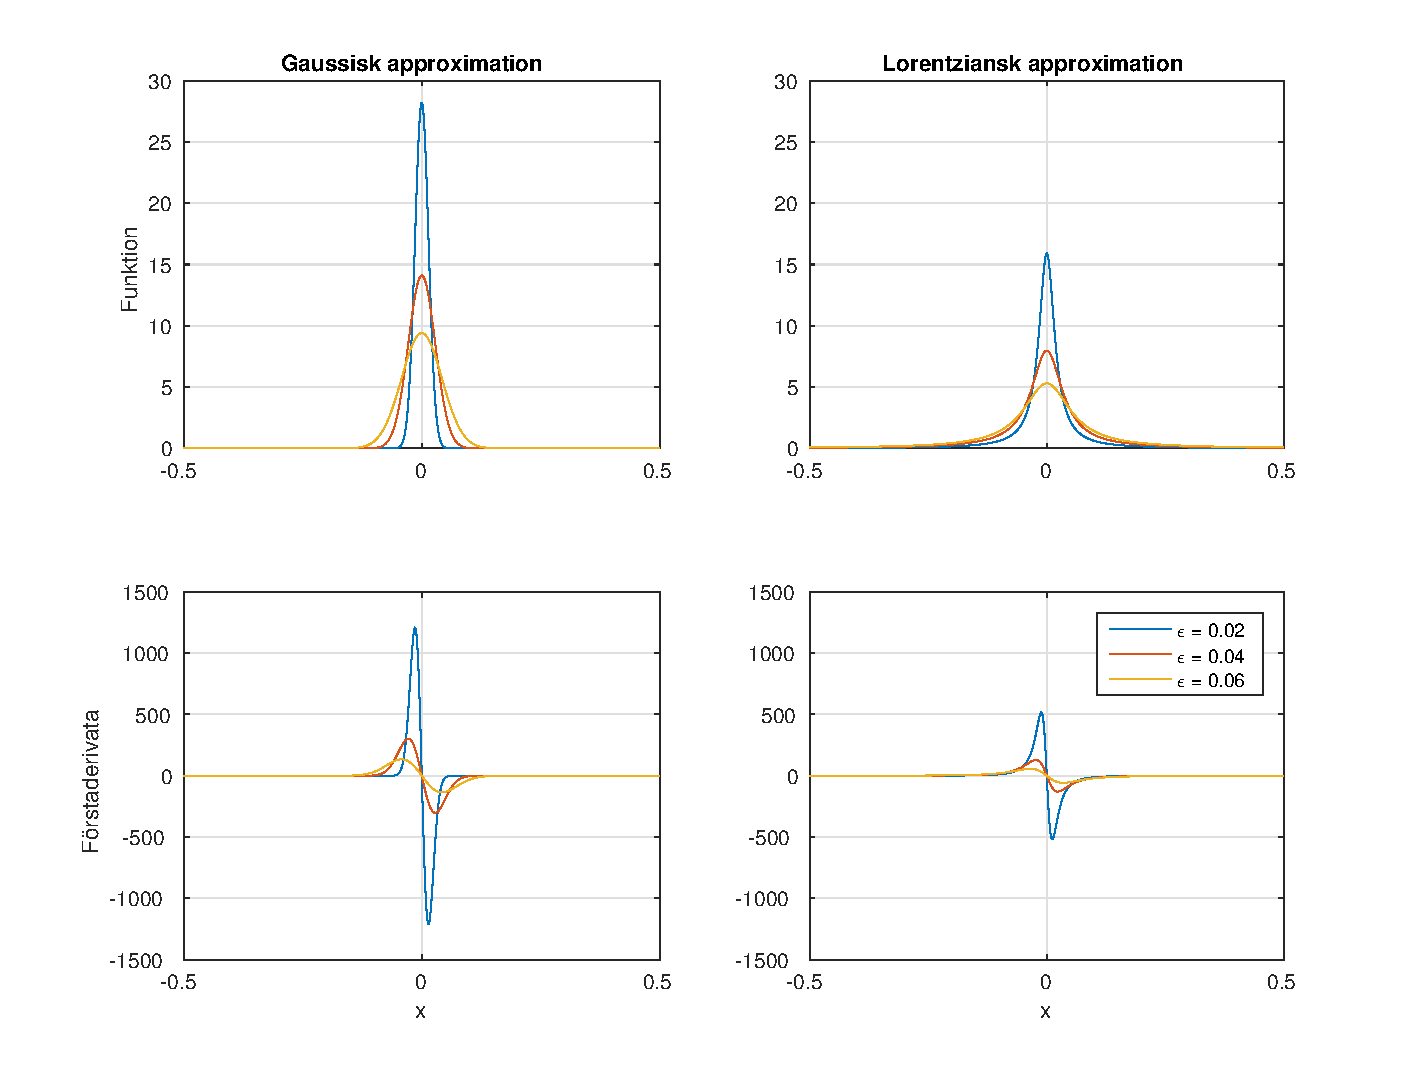
\includegraphics[width=0.9\linewidth]{fig/fig721.pdf}}
  \caption{
  Två distributioner och deras förstaderivator i gränsen $\epsilon \to 0$. \label{fig:71}
  }
\end{figure}
%\clearpage % flush figures fig:71



\begin{figure}[!ht]  % fig:72
  \centerline{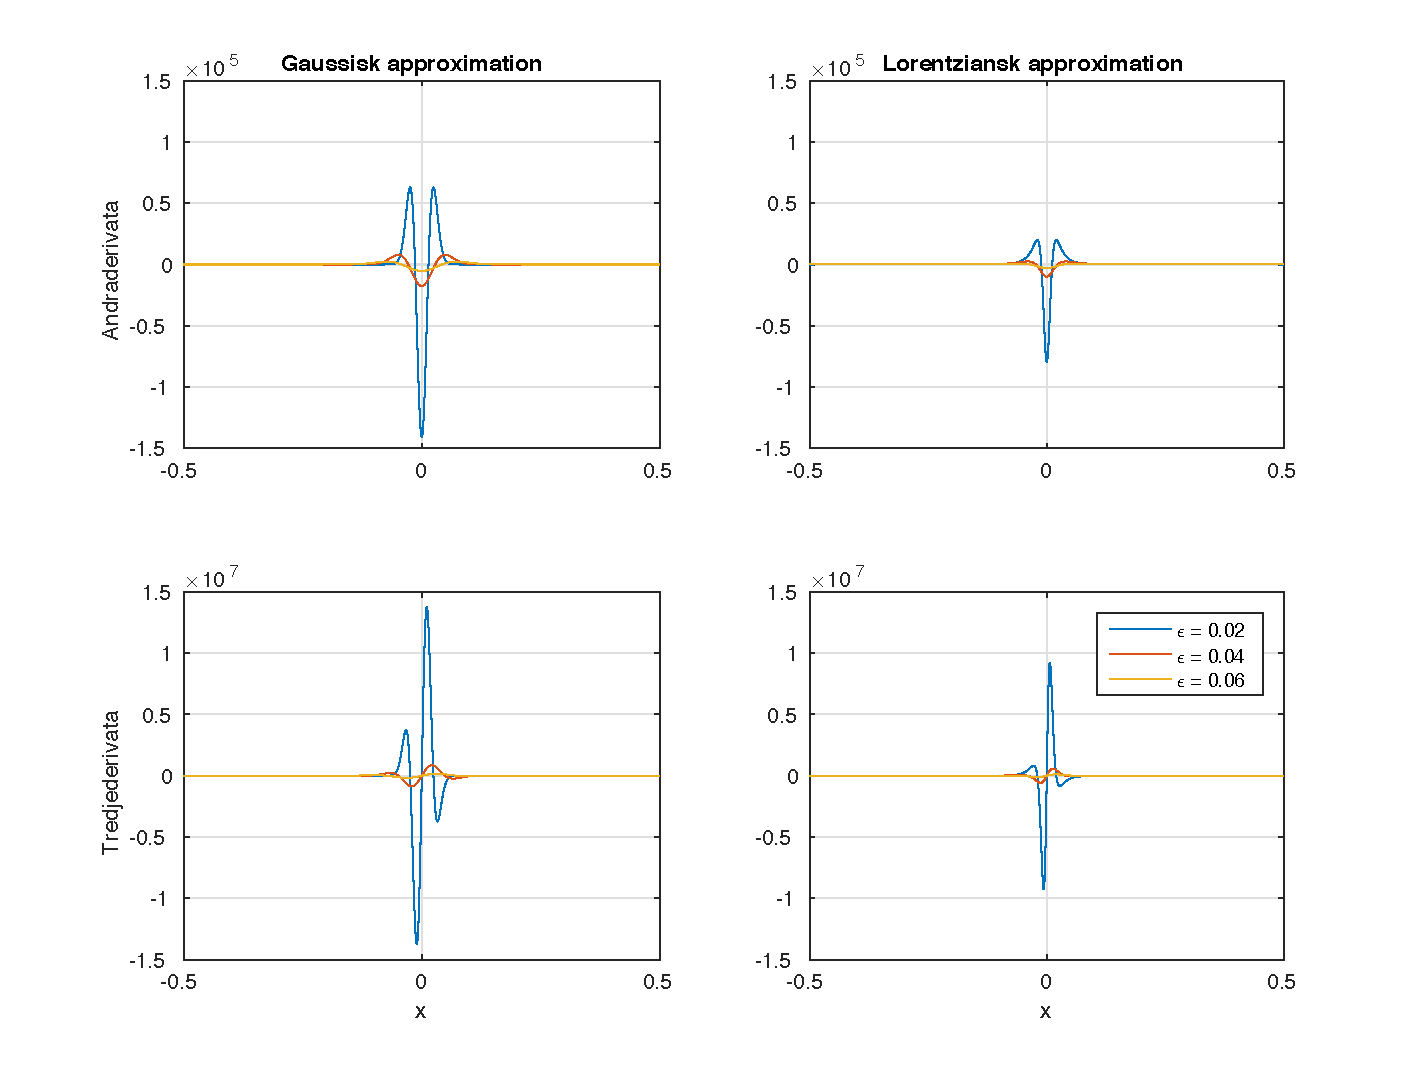
\includegraphics[width=0.9\linewidth]{fig/fig722.pdf}}
  \caption{
  Andra- och tredjederivator av två distributioner i gränsen $\epsilon \to 0$. \label{fig:72}
  }
\end{figure}
%\clearpage % flush figures fig:72


Deltafunktionens derivator ska gå att partialintegrera (se diskussionen av ekvation (7.9) i kurskompendiet). Det vill säga (alla integraler går över hela $\mathbb R$, så alla randtermer är lika med noll):
\begin{align}
    \int \mathrm dx\ \delta'(x)f(x)&=-\int \mathrm dx\ \delta(x)f'(x)=-f'(0),\\
    \int \mathrm dx\ \delta''(x)f(x)&=\int \mathrm dx\ \delta(x)f''(x)=f''(0),\\
    \int \mathrm dx\ \delta'''(x)f(x)&=-\int \mathrm dx\ \delta(x)f'''(x)=-f'''(0).
    \label{eq:tredje}
\end{align}

\paragraph{Explicit integrering.}
Låt oss visa detta explicit för de två distributionerna som betraktas här. För en godtycklig slät funktion $f(x)$ kan vi Taylorutveckla:
\begin{equation}
    f(\epsilon)\approx f(0)+f'(0)x+\frac12f''(0)x^2+\frac16f'''(0)x^3+\ldots.
\end{equation}
I båda fallen ovan är $h_\epsilon(x)$ en jämn funktion, så alla termer av typen $x^{2n+1}h_\epsilon(x)$, $n\in\mathbb Z$ integreras till noll. 

Vi börjar titta på den Gaussiska approximationen. Inför notationen $f^{(n)}(0)\equiv f^{(n)}_0$. För förstaderivatan får vi följande genom att utföra integralerna (se formelsamling) eller genom att partialintegrera upprepade gånger,
\begin{align}
    \int\mathrm dx\ f(x)h'_\epsilon(x)&\approx-\frac{2}{\epsilon^2}\int\mathrm dx\ xh_\epsilon(x)\left[f'_0x+\frac16f'''_0x^3+\ldots\right] \nonumber\\
    &=-f'_0-\frac14f'''_0\epsilon^2+\ldots.
\end{align}
Det är lätt att inse att alla termer som innehåller högre ordningens derivator  av $f(x)$ kommer vara proportionella mot $\epsilon$, och gå mot noll. Kvar finns bara den väntade $-f'(0)$.

På samma sätt studerar vi integralen över andraderivatan:
\begin{align}
    \int\mathrm dx\ f(x)h''_\epsilon(x)&\approx\int\mathrm dx\ \frac{4x^2-2\epsilon^2}{\epsilon^4}h_\epsilon(x)\left[f_0+\frac12f''_0x^2+\ldots\right] \nonumber\\
    &=\frac{2-2}{\epsilon^2}f(0)+\frac{3-1}2f''_0 + \epsilon^2 [\ldots].
\end{align}
De högre ordningens termer kommer återigen vara proprotionella mot $\epsilon$, och försvinner när gränsvärdet tas, vilket resulterar i att bara $f''(0)$ finns kvar.

Vi övergår nu till att studera den Lorentzianska approximationen. På samma sätt som ovan får vi för förstaderivatan
\begin{gather}
    \int\mathrm dx\ f(x)h'_\epsilon(x)\approx-\int\mathrm dx\ \frac{2 x}{x^2+\epsilon^2}h_\epsilon(x)\left[f'_0x+\frac16f'''_0x^3+\ldots\right] \nonumber\\
    =-f'_0-\frac\epsilon{3\pi}\left[x+\frac{\epsilon^2x}{2\epsilon^2+2x^2}-\frac{3\epsilon}2\tan^{-1}\frac x\epsilon\right]_{-\infty}^\infty+\ldots.
\end{gather}
Eftersom att $x$ här är en integrationsvariabel har den inget konstigt för sig, utan går linjärt mot oändligheten. I gränsen $\epsilon\rightarrow 0$ går därför de högre ordningens termer mot noll, och vi får igen det väntade resultatet. 

För andraderivatan får vi
\begin{gather}
    \int\mathrm dx\ f(x)h''_\epsilon(x)\approx\int\mathrm dx\ \frac{6x^2-2\epsilon^2}{\left(x^2+\epsilon^2\right)^2}h_\epsilon(x)\left[f_0+\frac12f''_0x^2+\ldots\right] \nonumber\\
    =\frac{3-3}{4\epsilon^2}f(0)+\frac{9-1}8f''_0 + \epsilon [\ldots]
\end{gather}
där alltså högre ordningens termer är proportionella mot $\epsilon$.

Att bevisa ekvation (\ref{eq:tredje}) för de båda fallen av $h_\epsilon(x)$ lämnas som en övning.

\paragraph{Resonemang utgående från funktionernas form.}
Vi kan också resonera utgående från figurerna~\ref{fig:71} och~\ref{fig:71} varför vi får dessa resultat. För att göra detta drar vi oss först till minnes uttrycken för olika ordningars derivator i termer av finita differenser:
\begin{align}
f'(x) &= \lim_{\epsilon \to 0} \frac{f(x+\epsilon/2)-f(x-\epsilon/2)}{\epsilon} \\
f''(x) &= \lim_{\epsilon \to 0} \frac{f(x+\epsilon)-2f(x)+f(x-\epsilon)}{\epsilon^2} \\
f'''(x) &= \lim_{\epsilon \to 0} \frac{f(x+3\epsilon/2)-3f(x+\epsilon/2)+3f(x-\epsilon/2)-f(x-3\epsilon/2)}{\epsilon^3}.
\end{align}
Det är inte svårt att föreställa sig att förstaderivatorna som ritats upp i den andra raden av figur~\ref{fig:71} kommer att plocka upp $-f(0+\epsilon/2)$ och $+f(0-\epsilon/2)$. Notera också att amplituden på de två topparna är lika stor och växer som $1/\epsilon$. Resultatet motsvarar alltså den finita differensen som definierar förstaderivatan av en funktion $f(x)$ i punkten $x=0$, fast med motsatt tecken.

På liknande sätt kan vi resonera kring de högre ordningarnas derivator och jämföra figurerna med uttrycken från finita differenser. Notera speciellt den relativa storleken på de olika topparna och att amplituderna blir högre för andraderivatorna ($\sim 1/\epsilon^2$) och ännu högre för tredjederivatorna ($\sim 1/\epsilon^3$).

% --- end solution of exercise ---

\end{doconceexercise}
% --- end exercise ---


% ------------------- end of main content ---------------

\end{document}

